\documentclass[11pt,twocolumn]{article}

\usepackage[utf8]{inputenc}
\usepackage[numbers]{natbib}
\usepackage[T1]{fontenc}
\usepackage{textcomp}
\usepackage{amsmath, amssymb}
\usepackage{mdframed}
\usepackage{pgfplots}
\usepackage{import}
\usepackage{mathrsfs}
\usepackage{hyperref}
\usepackage{xifthen}
\usepackage{float}
\usepackage{nicematrix}
\usepackage{pdfpages}
\usepackage{tcolorbox}
\usepackage{transparent}
\usepackage{geometry}
\usepackage{lipsum}
\pgfplotsset{compat=1.18}
\usepackage{tikz}
\usetikzlibrary{shapes.misc}
\newtheorem{theorem}{Theorem}{}
\newtheorem{corollary}{Corollary}{}
\newtheorem{remark}{Remark}{}

% change margins
\geometry{top=2cm, bottom=3cm, left=2.5cm, right=2.5cm}
% space after section
\usepackage{titlesec}
\titlespacing*{\section}{0pt}{0.5\baselineskip}{0.5\baselineskip}
\titlespacing*{\subsection}{0pt}{0.5\baselineskip}{0.5\baselineskip}
\titlespacing*{\subsubsection}{0pt}{0.5\baselineskip}{0.5\baselineskip}
\renewcommand\thesection{\arabic{section}.}

\setlength{\columnsep}{2em}
\hypersetup{hidelinks}
\usetikzlibrary{arrows, arrows.meta}

\tikzset{cross/.style={cross out, draw=black, minimum size=2*(#1-\pgflinewidth), inner sep=0pt, outer sep=0pt, style = ultra thick},
%default radius will be 1pt. 
cross/.default={5pt}}

% figure support
\usepackage{import}
\usepackage{xifthen}
\usepackage{collectbox}
\usepackage{enumerate}
\usepackage{amsfonts}
\pdfminorversion=7
\usepackage{pdfpages}
\usepackage{transparent}
\newcommand{\incfig}[1]{%
	\def\svgwidth{\columnwidth}
	\import{./figures/}{#1.pdf_tex}
}
\usepackage{fancyhdr}

\begin{document}

\title{Streamlining Inventory Management for Storable Healthcare Products in a Unified Demand Environment}

\author{Nathaniel Mitrani, Alex Serrano, Jan Tarrats, Joel Solé\\ Polytechnic University of Catalonia}

\maketitle

\begin{abstract}
	In this project, we propose a mathematical model and implementation based on a collaborative scheme designed to optimize the storage and distribution of medical products to hospitals given historical data.
\end{abstract}

\section{Introduction}\label{sec1}
Supply chain robustness is of paramount importance for businesses, as it not only ensures operational continuity but also provides significant financial benefits. Especially in medical settings, robustness is imperial as the effects of a shortage can cost human lives \cite{key3}.
Additionally, it is of paramount importance for a company to minimize the ecological footprint stemming from its activities, especially related to transportation which is a major source of pollution, 28\% as of 2021 \cite{key1}.

\section{Problem Statement}\label{sec2}
The goal is therefore to find cost-optimality whilst satisfying robustness and environmental constraints. We suggest a unified demand approach to tackle the problem, that is an agreement reached by an array of medical institutions to combine the demand for medical products in one single order to reduce cost \cite{key2}, followed by a mathematical model and further implementation to solve the problem in this setting. For simplicity, we consider a time granularity of months.

\section{Proposed solution}\label{sec3}
In the unified demand scenario, we assume that all the hospitals group their orders for a given product in one order, with the referenced economical benefits that this supposes \cite{key2}. We consider therefore each product separately and build a model to optimize the processes for each product.

Given a specific product, we consider a unique provider and distribution center (as we are in a given region we can assume a certain locality). Our challenge is to optimize the costs given a certain environmental footprint and resilience score.

We quantify the environmental impact as proportional to the number of orders, as referenced in \cite{key1} and in the problem specification. This amounts to choosing when and how much to order given robust satisfaction of demand, fixed number of orders, and storage costs.

The demand we obtain comes from a prediction for the purchase plan, from which we yield the amount of units needed for the coming year.

\begin{figure}[h]
	\centering
	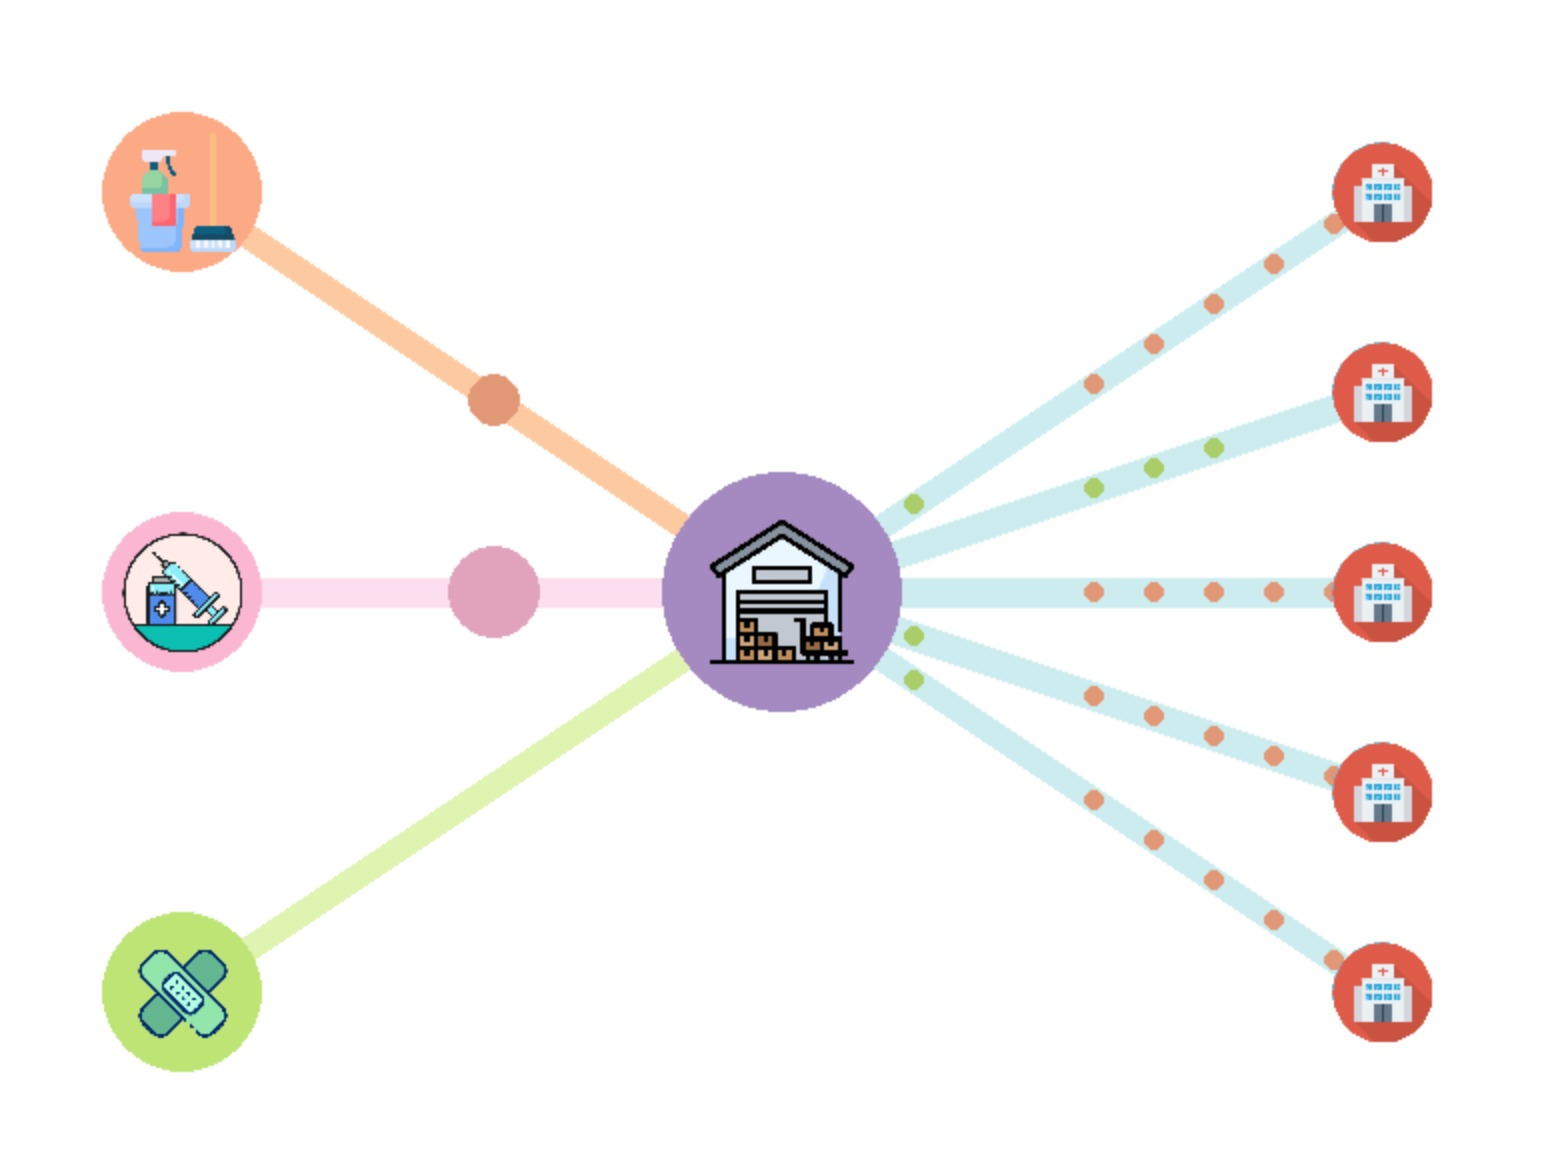
\includegraphics[width=8cm]{WhatsApp Image 2023-11-12 at 01.28.21.jpeg}
	\caption{Image showing concatenation of 3 models (3 products), assuming that the distribution centers for each product are in the same location (graphical purposes)}
	\label{fig:enter-label}
\end{figure}

\section{Modelling product demand}
Our goal here is to establish the optimal offer (amount of units) for a given product throughout 2023, as a byproduct of creating a demand predictor that uses historical data.

\subsection{Model evaluation}
First, we establish the metrics that are going to be used to evaluate, compare and select models.

\subsubsection{Tweedie loss}
The Tweedie loss, as presented in Zhou, He et al. \cite{key5}, provides a way to measure goodness of fit of a forecasting model. It is robust to skewed distributions, as is the case in the dataset. The metric range is $(-\infty, 1]$, where $-\infty$ is a completely random model, 0 is a model that always predicts the empirical mean of a times series and 1 is an exact prediction.

\subsubsection{Expense MAPE}
To allow the less-technical users of the model to be able to interpret the error with its real-life repercussions, we report the mean absolute percent error in predicted expenses for 2023 by product. That is, the mean of the percentual absolute error between the real expenses and the predicted expenses for 2023.

\subsection{Models considered}
To allow for a diverse set of models, we have considered several families of predictors, specific forecasting models (Prophet, \cite{key6}), general regression models (GBMs, regularized polynomial regressions, Generalized Additive Models) and deep learning models (Seq2Seq \cite{key7}, Temporal Fusion Transformers \cite{key4}). In the following, we report the best two results.

\subsubsection{Boltzmann ensemble of GBMs}
A Boltzmann ensemble is an ensemble that uses a Boltzmann distribution to weight the predictions of the models in the ensemble. The Boltzmann distribution is a probability distribution that assigns a probability to each model in the ensemble, and the probability of a model is proportional to its performance on the validation set. The Boltzmann distribution is defined as follows:
\begin{equation*}
	P\left( m \right) = \frac{e^{-\frac{1}{T} \cdot \text{loss}\left( m \right) }}{\sum_{m' \in M}^{} e^{-\frac{1}{T} \cdot \text{loss}\left( m' \right) }}
\end{equation*}

Thus, the probability of a model is inversely proportional to its loss, and the temperature $T$ controls the variance of the distribution. The lower the temperature, the more the distribution is concentrated around the best model. We empirically choose a temperature of 0.1, which is a good compromise between variance and bias.

In terms of the individual models, we use a set of gradient boosted trees (XGBoost, CatBoost, HistGradientBoostedRegressors).

The results are shown in Table \ref{tab:enter-label}.

\subsubsection{Temporal Fusion Transformers}
The Temporal Fusion Transformer \cite{key4} is a novel attention-based architecture that combines high-performance multi-horizon forecasting with interpretable insights into temporal dynamics. To learn temporal relationships at different scales, TFT uses recurrent layers (LSTMs) for local processing and interpretable self-attention layers for long-term dependencies. TFT utilizes specialized components to select relevant features (variable selection networks) and a series of gating layers (with gated linear units) to suppress unnecessary components, enabling high performance in a wide range of scenarios.

We have employed our own implementation of the paper in PyTorch, and we have used the same hyperparameters as in the paper, that demonstrate a 36-69\% improvement over other deep forecasting learners such as DeepAR and NHiTS in standard benchmarks (see paper). The model has been trained in 1,5 GPU hours in an NVIDIA P100.

See the summary of the results in Table \ref{tab:enter-label}.

\begin{table}[h]
	\centering
	\begin{tabular}{|c|c|c|}
		\hline
		Model    & Tweedie & Expense MAPE \\
		\hline
		Ensemble & 0.70894 & 0.07146      \\
		\hline
		TFT      & 0.16871 & 0.2293       \\
		\hline
	\end{tabular}

	\caption{Metric results for presented models}
	\label{tab:enter-label}
\end{table}

\section{Mathematical formulation of the model}
\subsection{Model description}
\subsubsection{Sets of indices}
\begin{itemize}
	\item $I = \left\{ \text{index set for the product} \right\}, i \in I $
\end{itemize}

\subsubsection{Constants}
\begin{itemize}
	\item $c_i$: monthly storage cost for a unit of product  $i$.
	\item $C_{max}^{i}$: maximum quantity of product $i$ that we can store.
\end{itemize}

\subsubsection{Computed parameters}
\begin{itemize}
	\item  $v^{i}\left( t \right) $: consumption velocity of product $i$ at time  $t$
	\item $\xi^{i}\left( t \right) $: Demand checkpoint of unified demand at time $t$.
\end{itemize}


\subsubsection{Parameters of optimization}
\begin{itemize}
	\item $\beta$: Resilience factor, factor by which we multiply demand to increase supply chain resilience.
	\item  $P_{max}$ : Number of orders $\propto$ $CO_2$ emissions, a proxy for environmental impact.
\end{itemize}

\subsubsection{Variables}
\begin{itemize}
	\item $p^{i}\left( t \right) $ : quantity of product $i$ demanded at time  $t \in \left\{ 1,\ldots,12 \right\} $
	\item  $\delta\left( t \right) $: boolean (binary) variable to determine if there is an order at time \qquad \qquad $t \in \left\{ 1,\ldots,12 \right\} $
\end{itemize}

\subsubsection{Auxiliary variables}

\begin{remark}
	For simplicity and interpretability, we define this adjacent variable $s^{i}\left( t \right) $ corresponding to storage of product $i$ at the beginning of the time unit $t$.
\end{remark}

\begin{itemize}
	\item $s^{i}\left( t \right) = - \sum_{t'=1}^{t-1} v^{i}\left( t' \right)  + \sum_{t'=1}^{t} \delta\left( t' \right) \cdot p^{i}\left( t' \right)  $
\end{itemize}

\subsubsection{Constraints}

Capacity constraint:
\begin{align*}
	 & s^{i}\left( t \right) \le C^{i}_{max} \hspace{4mm} \forall t = 1,\ldots,12
	.\end{align*}

Sufficient inventory constraint:
\begin{align*}
	 & s^{i}\left( t \right) + \sum_{t'=1}^{t-1} v^{i}\left( t' \right) \ge \beta\cdot \sum_{t'=1}^{t} \xi^{i}\left( t' \right) \hspace{4mm} \forall t = 1,\ldots,12
	.\end{align*}


Environmental constraint ($P_{max}$ orders):
\begin{align*}
	 & \sum_{t=1}^{12} \delta\left( t \right) = P_{max}
	.\end{align*}

Variable domain constraint:
\begin{align*}
	 & s^{i}\left( t \right) \ge 0 \hspace{4mm} \forall t = 1,\ldots,12                       \\
	 & p^{i}\left( t \right) \ge 0 \hspace{4mm} \forall t = 1,\ldots,12                       \\
	 & \delta \left( t \right) \in  \left\{ 0,1 \right\} \hspace{4mm} \forall t = 1,\ldots,12
\end{align*}

\subsubsection{Objective function}
\hspace{4mm} $ f_i(\mathbf{p}) = \sum_{t}^{} s^{i}\left( t \right) \cdot c_i$

\subsection{Computation of parameters}
\subsubsection{Computing $\xi_i(t)$}
$\xi_i(t)$ is computed by cumulating all the purchased quantities of the product $i$ by all the hospitals predicted by our model in time step $t$.

\subsubsection{Computing $v_i(t)$}
$v_i(t)=\frac{\xi_i(t_-)}{t_+-t_-}$, where $t_-=\max\{t': 0\leq t'\leq t, \xi_i(t') \neq 0\}$, and $t_+=\min\{t':t<t'\leq 12, \xi_i(t')\neq 0\}$, i.e. $v_i(t)$ represents the slope between the previous purchase and the next, therefore supposing uniform consumption between orders, and complete depletion from one order to the next (i.e. the demand is perfectly predicted).


\section{Example: product 70130}

We have used different values for $\beta$ and $P_{max}$ to observe the effects of different environmental and robustness restrictions on the optimal cost of storage. As expected, the more robust and the fewer orders allowed (i.e. the less environmental impact) lead to increased optimal costs. We also observe that it is significantly harder to have a lesser environmental impact than to be more robust.

\begin{figure}[ht]
	\centering
	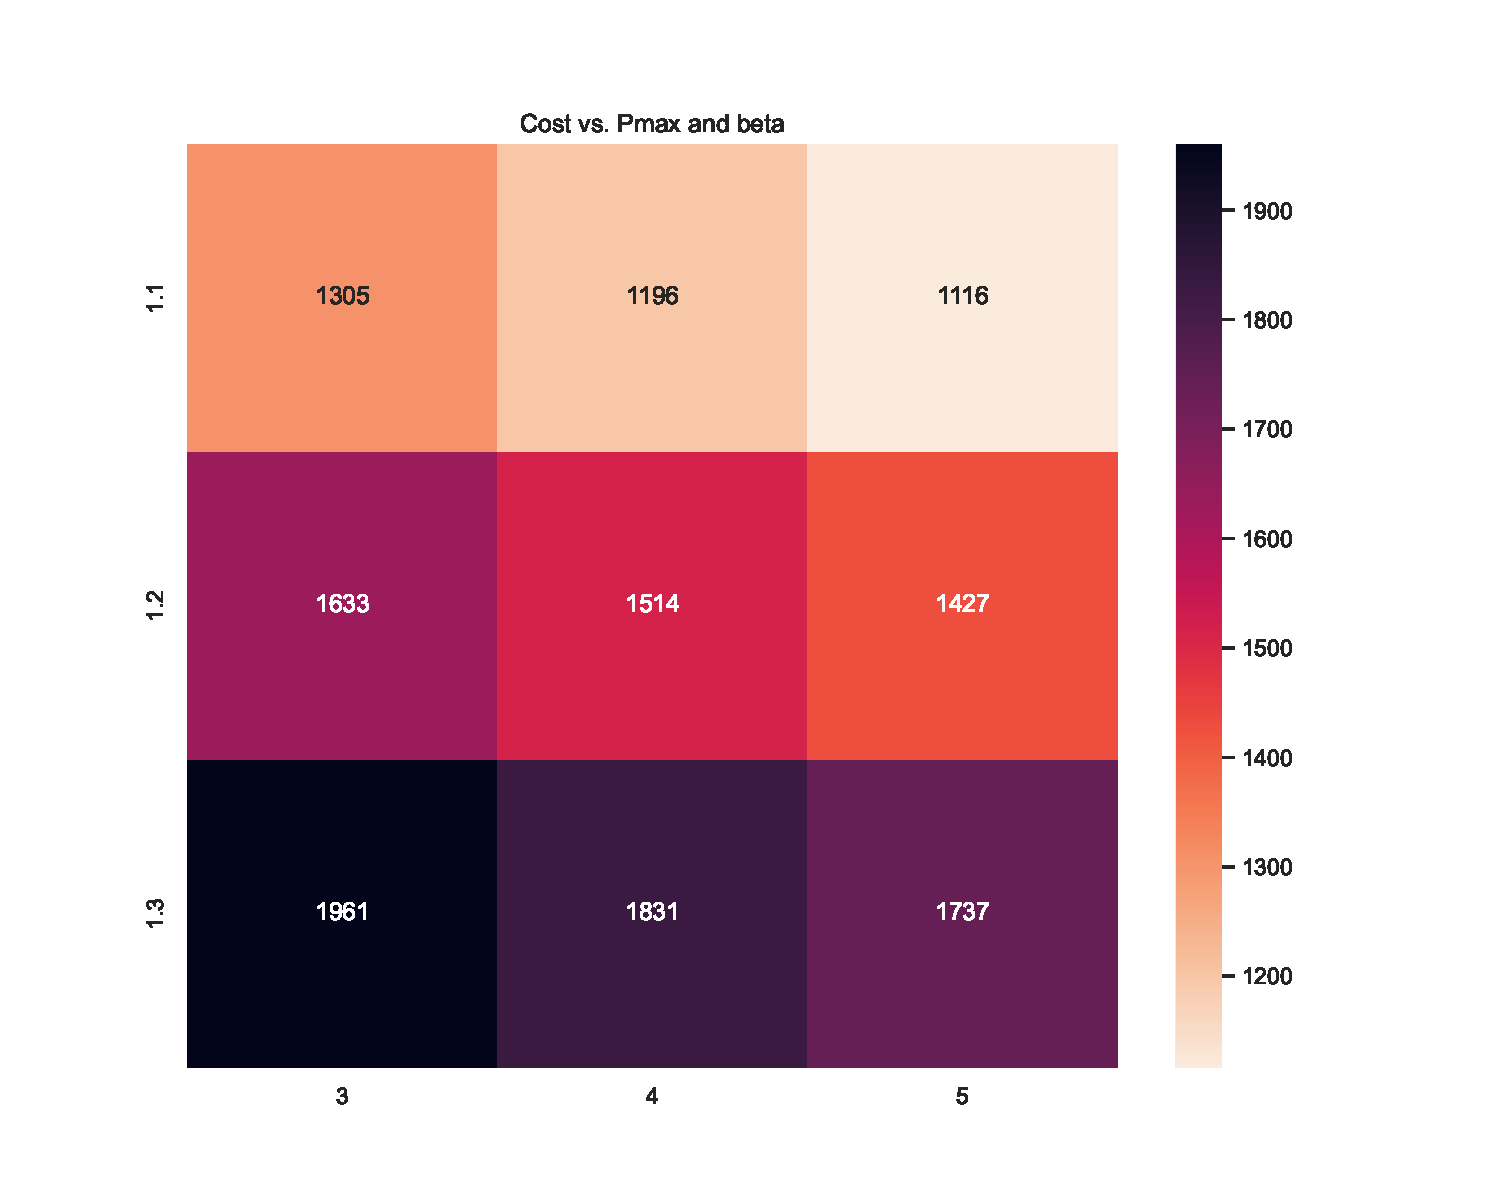
\includegraphics[width=9cm]{heatmap.pdf}
	\caption{Heatmap of optimal costs in terms of $\beta$ and $P_{max}$.}
	\label{fig:enter-label2}
\end{figure}


\section{Conclusions and future work}

In conclusion, our collaborative scheme and mathematical model offer a promising approach to optimize the storage and distribution of medical products in a unified demand scenario. The consideration of environmental impact and resilience scores in the optimization process aligns with the growing emphasis on sustainability and supply chain robustness. However, there are several avenues for improvement and future research that can enhance the effectiveness of our proposed solution.

One key area for improvement lies in refining the deep learning model used for predicting product demand. Our current approach relies on a predictive model for the purchase plan, which determines the quantity of units needed for the upcoming year. By incorporating more advanced deep learning techniques, such as recurrent neural networks or attention mechanisms, we can potentially enhance the accuracy of our demand predictions. This, in turn, would lead to more precise optimization of storage and distribution processes.

Furthermore, a deeper exploration into storage optimization processes could yield additional insights. Investigating advanced storage strategies, such as dynamic allocation algorithms or real-time inventory management, could contribute to further reducing costs and improving overall efficiency. Additionally, considering dynamic changes in demand patterns and adjusting storage strategies accordingly could enhance our model's adaptability to evolving scenarios.

In summary, future work should focus on enhancing the accuracy of demand predictions through advanced deep learning techniques and exploring advanced storage optimization strategies. By addressing these aspects, we can further advance the effectiveness of our proposed solution and contribute to the ongoing efforts in creating resilient, environmentally conscious supply chains for medical products.

\begin{thebibliography}{}
	\bibitem{key1} Sources of greenhouse gas emissions | US EPA. (n.d.). \url{https://www.epa.gov/ghgemissions/sources-greenhouse-gas-emissions }
	\bibitem{key2} L’ICS ESTALVIA 30,5 milions d’euros fent Compres Agregades. Institut Català de la Salut. (n.d.). \url{https://ics.gencat.cat/ca/detall/noticia/compres-agregades.html}
	\bibitem{key3} Phuong JM, Penm J, Chaar B, Oldfield LD, Moles R. The impacts of medication shortages on patient outcomes: A scoping review. PLoS One. 2019 May 3;14(5):e0215837. doi: 10.1371/journal.pone.0215837. PMID: 31050671; PMCID: PMC6499468.
	\bibitem{key4} Lim, Bryan \& Arık, Sercan \& Loeff, Nicolas \& Pfister, Tomas. (2021). Temporal Fusion Transformers for interpretable multi-horizon time series forecasting. International Journal of Forecasting. 37. 10.1016/j.ijforecast.2021.03.012.
	\bibitem{key5}{Zhou, He, et al. Tweedie Gradient Boosting for Extremely Unbalanced Zero-Inflated Data. arXiv, 14 Nov. 2019.}
	\bibitem{key6}{Sean J. Taylor, Benjamin Letham (2018) Forecasting at scale. The American Statistician 72(1):37-45 (https://peerj.com/preprints/3190.pdf)}
\end{thebibliography}

\end{document}

